\documentclass[12pt]{article}
\RequirePackage[l2tabu, orthodox]{nag}
\usepackage[main=english]{babel}
\usepackage[rm={lining,tabular},sf={lining,tabular},tt={lining,tabular,monowidth}]{cfr-lm}
\usepackage{amsthm,amssymb,latexsym,gensymb,mathtools,mathrsfs}
\usepackage[T1]{fontenc}
\usepackage[utf8]{inputenc}
\usepackage[pdftex]{graphicx}
\usepackage{caption}
\usepackage{subcaption}
\usepackage{epstopdf,enumitem,microtype,dcolumn,booktabs,hyperref,url,fancyhdr}
\usepackage{tikz}
\usetikzlibrary{positioning}

% Plotting
\usepackage{pgfplots}
\usepackage{xinttools} % for the \xintFor***
\usepgfplotslibrary{fillbetween}
\pgfplotsset{compat=1.8}
\usepackage{tikz}

% Custom Commands
\newcommand*{\norm}[1]{\left\lVert#1\right\rVert}
\newcommand*{\abs}[1]{\left\lvert#1\right\rvert}
\newcommand*{\suchthat}{\,\mathrel{\big|}\,}
\newcommand{\E}{\mathbb{E}}
\newcommand{\Var}{\mathrm{Var}}
\newcommand{\R}{\mathcal{R}}
\newcommand{\N}{\mathcal{N}}
\newcommand{\Ker}{\mathrm{Ker}}
\newcommand{\Cov}{\mathrm{Cov}}
\newcommand{\Prob}{\mathbb{P}}
\DeclarePairedDelimiterX\innerp[2]{(}{)}{#1\delimsize\vert\mathopen{}#2}
\DeclareMathOperator*{\argmax}{argmax}
\DeclareMathOperator*{\argmin}{argmin}
\def\R{\mathbb{R}}
\DeclarePairedDelimiter\ceil{\lceil}{\rceil}
\DeclarePairedDelimiter\floor{\lfloor}{\rfloor}

\setlist{topsep=1ex,parsep=1ex,itemsep=0ex}
\setlist[1]{leftmargin=\parindent}
\setlist[enumerate,1]{label=\arabic*.,ref=\arabic*}
\setlist[enumerate,2]{label=(\alph*),ref=(\alph*)}

% Specifically for paper formatting 
\renewcommand{\baselinestretch}{1.2} % Spaces manuscript for easy reading

% Formatting definitions, propositions, etc. 
\newtheorem{definition}{Definition}
\newtheorem{prop}{Proposition}
\newtheorem{lemma}{Lemma}
\newtheorem{thm}{Theorem}
\newtheorem{corollary}{Corollary}
\newtheorem{notation}{Notation}

\begin{document}

\begin{center}
\Large
Basics of Neural Networks 
\end{center}

\begin{flushright}
Andrew Roberts
\end{flushright} 

\section{Introduction}
The neural network era has expanded many of the ideas from the Generalized Linear Models (GLMs) that preceded it. As the amount and complexity and data has continued 
to grow, the desire for more ``expressive'' models has also increased; that is, the ability to model more complex relationships with a broader class of functional forms. GLMs are 
quite flexible and still widely used, but neural networks are able to tackle even more complex problems. In fact, the first major theorem of neural networks is that they are 
``universal function approximators''; informally, given a large enough neural network one can approximate any function arbitrarily well. I hope to offer a brief introduction to neural 
networks here from the perspective of someone coming from a statistical modeling (linear models, GLMs, etc.) perspective in order to remove some of the mystery of this class 
of models. Indeed, we will see that neural networks simply re-package and expand many of the core ideas of GLMs. The resulting class of models is certainly more complex, but the 
core ideas remain largely the same. 

\section{The Basic Setup}
The basic learning-theoretic setup is as follows. We consider an input space $\mathcal{X}$ (features/attributes/predictors) and an output space $\mathcal{Y}$ (responses/labels)
and we seek to learn a mapping $h: \mathcal{X} \to \mathcal{Y}$. In the statistical setting, the motivation for learning this mapping is often to be able to understand the relationship
between these spaces, to gain an understanding of how the explanatory variables are related to the response. As we will see, neural networks are a ``black box'' model in the sense 
that it is very difficult to gain an understanding of the relationships encoded by the model. Thus, the main motivation for neural networks is \textit{prediction}, to predict the value of the 
response given a feature vector. 

\subsection{Hypothesis Class}
Now, to learn a mapping between these spaces we of course need some data. Therefore, our setup assumes that we have access to training data
\[\mathcal{D} = \{(x_i, y_i) \in \mathcal{X} \times \mathcal{Y}: i = 1, \dots, N\}\]
Given this training data, trying to find the ``best'' mapping out of all possible functions is not very helpful. Of course we can simply define a function that correctly predicts every example
in the training data, but this will be overfitting to the training data and likely not generalize well to other datasets. Therefore, we restrict our attention to a set of possible mappings (i.e. models), 
which we call the \textit{hypothesis} class. In linear models, the hypothesis class is just the set of all linear functions of the inputs.
\[h_w(x) = x^T w\]
which simplifies the estimation step in the sense that all we need to optimize is the vector of regression coefficients $w$.
GLMs expand this hypothesis class by introducing non-linearities in the form of a link function $g$. 
\[h_w(x) = g^{-1}(x^T w)\]
Neural networks take this a step further. At the core will still be the notion of linearity; that is, the idea that the linear combination $x^T w$ acts as a summary of the input data. The leap is in the 
idea of letting the model find its own features. In the above examples, we feed the model features $x$, then we summarize them via $x^T w$, and in the case of GLMs potentially allow for 
non-linearity $g^{-1}(x^T w)$. What if we repeated this procedure various times? Ignoring non-linearity for the time being, we might consider something like
\[h(x) = W_2 W_1 x = W_2 (W_1 x)\]
We can think of the first layer $z := W_1 x$ as forming linear combinations of the given feature $x$, thus finding \textit{new} features that may be better than the given ones. Then the 
remaining layer $h(z) = W_2 z$ just looks like a typical linear model as a function of the newly discovered feature vector $z$. Intuitively, if we added more and more layers we would expect 
the model to be able to find complicated features, and thus to be more expressive. On the downside, we clearly have many more parameters to optimize now: every entry of the matrices $W_1$
and $W_2$. Throughout these notes we will denote by $\theta$ the vector of all parameters. So in this case $\theta = (W_1, W_2)$, where we can think of the matrices as being flattened into the 
vector $\theta$. To make the above model more flexible, we can introduce non-linearity. To do so we consider functions $f_1, f_2: \R \to \R$ and consider
\[h_\theta(x) = f_2(W_2 f_1(W_1 x))\]
where $f_1(W_1 x)$ means that $f$ is applied element-wise to each component of the vector $W_1 x$, and likewise for $f_2$. This is typically visualized as directed acyclic graph. Suppose 
$x \in \R^p$, $W_1 \in \R^{k \times p}$, $W_2 \in \R^{1 \times k}$. For simplicity, we are assuming that the function outputs a scalar value, which would be suitable for a binary classifier or a regression
problem. To generalize to multi-class problems we could assume that the model outputs a vector. 


\tikzset{%
  every neuron/.style={
    circle,
    draw,
    minimum size=1cm
  },
  neuron missing/.style={
    draw=none, 
    scale=4,
    text height=0.333cm,
    execute at begin node=\color{black}$\vdots$
  },
}

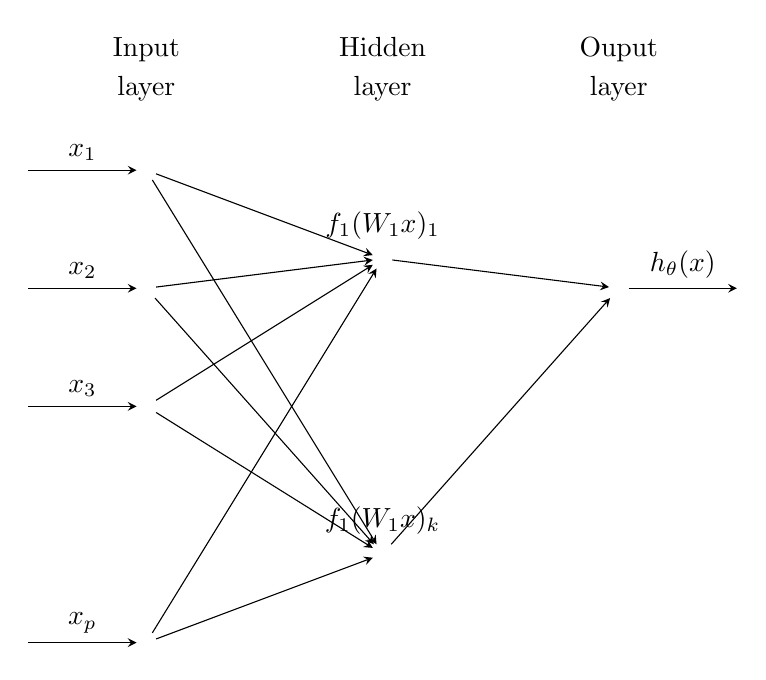
\begin{tikzpicture}[x=1.5cm, y=1.5cm, >=stealth]

\foreach \m/\l [count=\y] in {1,2,3,missing,4}
  \node [every neuron/.try, neuron \m/.try] (input-\m) at (0,2.5-\y) {};

\foreach \m [count=\y] in {1,missing,2}
  \node [every neuron/.try, neuron \m/.try ] (hidden-\m) at (2,2-\y*1.25) {};

\foreach \m [count=\y] in {1}
  \node [every neuron/.try, neuron \m/.try ] (output-\m) at (4,1.5-\y) {};

\foreach \l [count=\i] in {1,2,3,p}
  \draw [<-] (input-\i) -- ++(-1,0)
    node [above, midway] {$x_\l$};

\foreach \l [count=\i] in {1,k}
  \node [above] at (hidden-\i.north) {$f_1(W_1 x)_\l$};

\foreach \l [count=\i] in {1}
  \draw [->] (output-\i) -- ++(1,0)
    node [above, midway] {$h_\theta(x)$};

\foreach \i in {1,...,4}
  \foreach \j in {1,...,2}
    \draw [->] (input-\i) -- (hidden-\j);

\foreach \i in {1,...,2}
  \foreach \j in {1}
    \draw [->] (hidden-\i) -- (output-\j);

\foreach \l [count=\x from 0] in {Input, Hidden, Ouput}
  \node [align=center, above] at (\x*2,2) {\l \\ layer};

\end{tikzpicture}

\bigskip

Thus, we can think of each entry in $W_1$, $W_2$ as weighting a particular edge in the above graph, while the non-linearities are introduced by applying the function $f$ at the nodes
of the graph. In particular, $(W_\ell)_{ij}$ is the weight on the edge coming from the $j^{\text{th}}$ node of the $\ell^{\text{th}}$ layer and connecting to the $i^{\text{th}}$ node of the 
subsequent layer. With this basic example as motivation, we now introduce the hypothesis class used by neural networks. Neural networks consider all functions $h_\theta: \R^d \to \R$
defined recursively as follows. 
\begin{align*}
&z^{(1)} = x \qquad z^{(i)} = f_{i - 1}(W^{(i - 1)} z^{(i - 1)}) \ \forall i = 2, \dots, d \qquad h_\theta(x) = z^{(d)}
\end{align*}
where $\theta = (W_1, \dots, W_{d - 1})$. Note that this is exactly like the example $h_\theta(x) = f_2(W_2 f_1(W_1 x))$ considered above except we allow for an arbitrary number 
$d$ of layers ($d = 4$ would look like $f_3(W_3f_2(W_2 f_1(W_1 x)))$, etc.). 


\subsection{Loss Functions}
We've thus far neglected to talk about one key ingredient: the loss function. I've referred to optimizing $\theta$, but optimize with respect to what? In general, we define a loss function
\[\ell: \mathcal{X} \times \mathcal{Y} \to \R_+\]
such that $\ell(h_\theta(x), y)$ measures how far the prediction $h_\theta(x)(x)$ is from the true value $y$. Linear regression typically uses the $\ell_2$ squared loss
\[\ell(h_\theta(x), y) = (x^T w - y)^2\]
while in general GLMs minimize the negative log-likelihood, which leads to a variety of different loss functions. For neural networks a wide variety of loss functions are used. 

\subsubsection{Common Loss Functions}
\textbf{TODO: go through common loss functions here, starting with 0/1 loss, then hinge, etc.; showing how each is a more smooth version of the last}

\subsubsection{Training a Neural Network}
``Training'' a neural network refers to learning/optimizing the parameters $\theta$ with respect to the loss function and a giving training data set. In particular, the parameters are chosen 
as those that minimize the average loss over the training data. 
\[\hat{\theta} := \argmin_{\theta} \frac{1}{N} \sum_{i = 1}^{N} \ell(h_\theta(x_i), y_i)\]
In general, minimizing this function is not easy; this is the subject of the next section. 

% Section: Backpropagation
\section{Backpropagation}
If we assume that the loss function is differentiable, then the natural optimization approach is to calculate the gradient, set it equal to $0$, and solve for the parameters. 
\[\nabla_\theta \frac{1}{N} \sum_{i = 1}^{N} \ell(h_\theta(x_i), y_i) = 0\]
However, there is no way we're solving this explicitly; this could be a massive system of non-linear equations. The typical approach is thus to approximate the minimum via 
some iterative method, which typically comes in the form of a gradient descent-type approach. Therefore, the key step in being able to optimize a neural network is being able 
to calculate the gradient $\nabla_\theta \ell(h_\theta(x), y)$. At first glance, this might seem very difficult; $h_\theta(x)$ is this crazy-looking function defined recursively. However, 
when you have a composition of functions and want to take the derivative, you should immediately be thinking chain rule. That's pretty much all there is to this; it's just one big
chain rule calculation, which will yield the gradient that can then be used in gradient descent. Really the most difficult thing here is keeping track of notation. We will also 
detail some computational tricks that prevent having to calculate the same terms multiple times. The resulting method that is essentially just the chain rule with these computational 
tricks is called the \textit{backpropagation algorithm}. For those who have had experience with GLMs and Fisher Scoring/Iteratively Re-Weighted Least Squares, the mechanics of this 
will feel very familiar. In that case we wanted to apply Newton's method, and the bulk of the work was a large chain rule gradient calculation for the log-likelihood. The idea is quite similar
here. 

\subsection{Applying the Chain Rule}


\section{Connections between Neural Networks and GLMs}
\textbf{TODO}\\
See paper: From Generalized Linear Models to Neural Networks, and Back


\end{document}






